\appendix
\chapter{Pressure versus model-level interpolation}
% remove comment if you wish to add Appendix to contentsline.
%\addcontentsline{toc}{chapter}{Appendix A: How to download ERA5 data}
\section{Temperature}
\begin{figure}
    \centering
    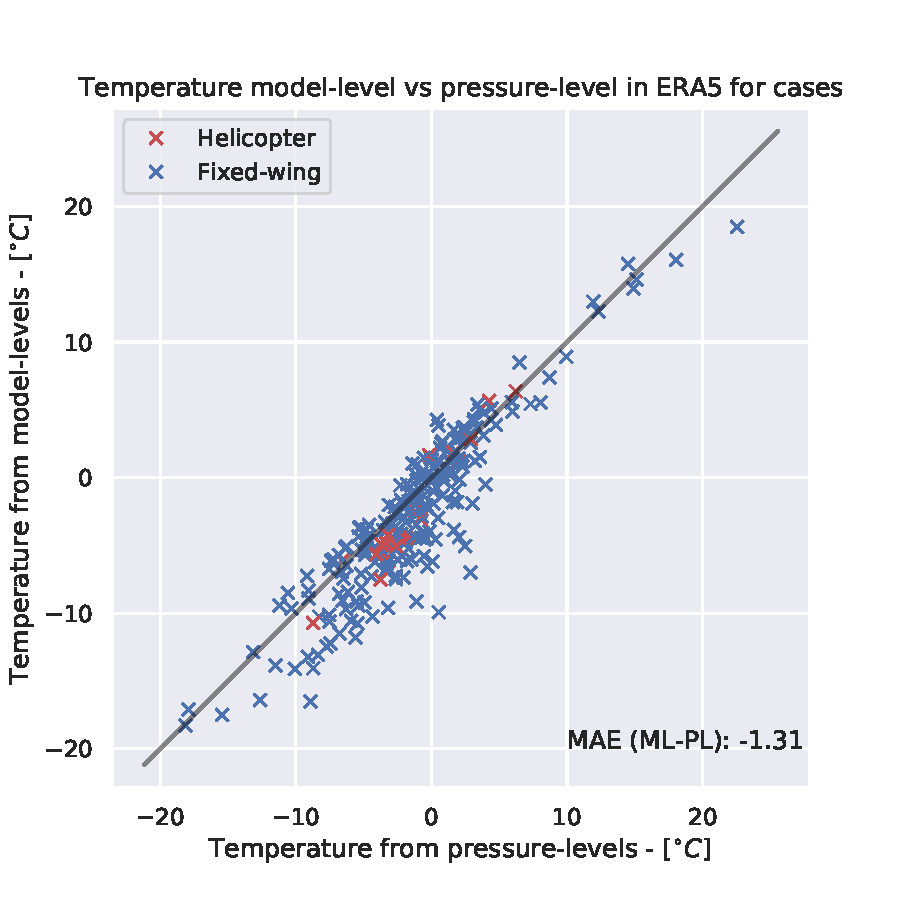
\includegraphics[width=0.8\textwidth]{Figures/mlvspl.pdf}
    \caption{Correlation between model-level and pressure-level interpolation of temperature from ERA5}
    \label{fig:mlvspl}
\end{figure}

\begin{figure}
    \centering
    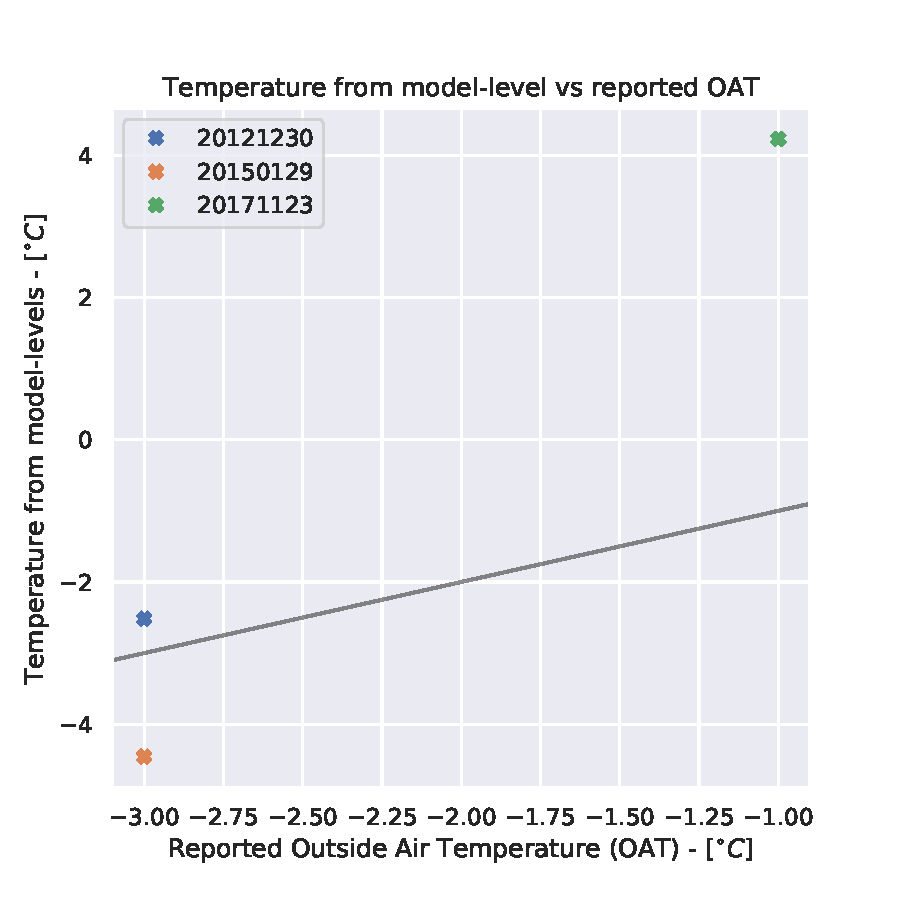
\includegraphics[width=0.5\textwidth]{Figures/mlvsoat.pdf}
    \caption{Correlation between model-level interpolation of temperature from ERA5 and observed Outside Air Temperature}
    \label{fig:mlvsoat}
\end{figure}

\begin{figure}
    \centering
    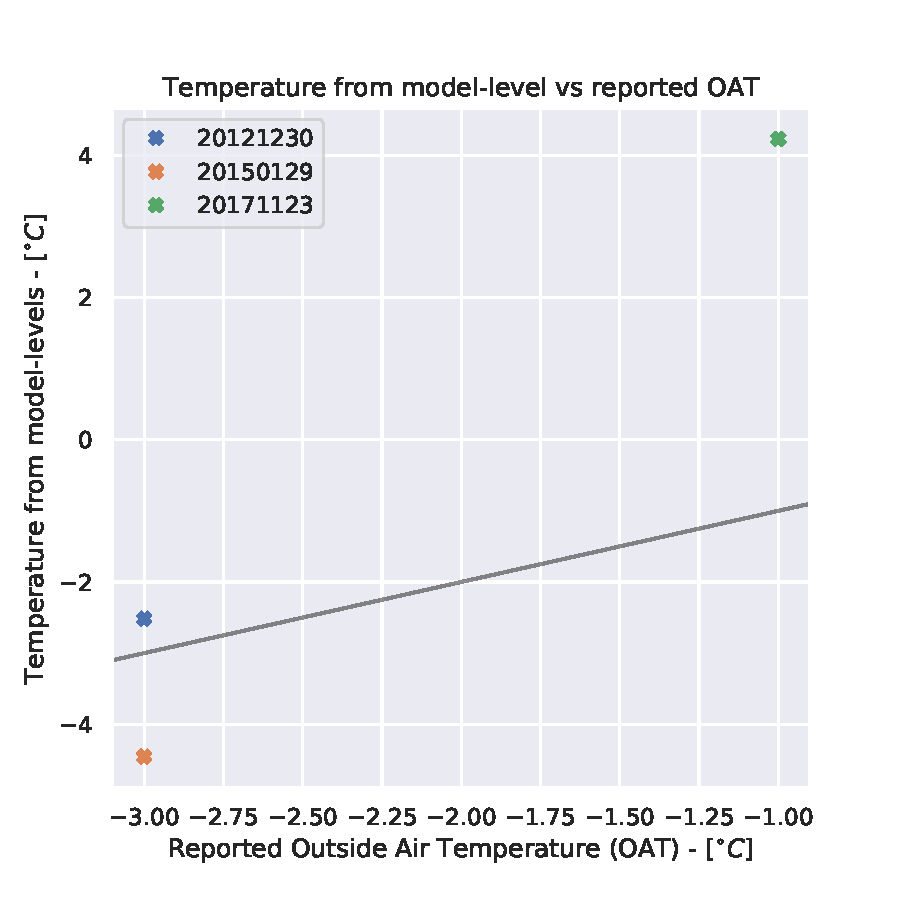
\includegraphics[width=0.5\textwidth]{Figures/mlvsoat.pdf}
    \caption{Correlation between pressure-level interpolation of temperature from ERA5 and observed Outside Air Temperature}
    \label{fig:plvsoat}
\end{figure}


\chapter{Operational categories of HTL-severity}
%\addcontentsline{toc}{chapter}{Appendix B: Additional figures}

